\chapter{Исследовательский раздел}

Предметом исследований является скорость и пропускная способность сервера при запросе картинки. Нагрузочное тестирование проводилось на примере изображения в формате JPG размером 100613 байт. Сравнивались разработанный сервер и Nginx~\cite{dejonghe2020nginx}.

Характеристики устройства, на котором проводилось исследование, следующие~\cite{macbook}:

\begin{itemize}
	\item оперативная память 16Гб;
	\item процессор Apple M1 Pro;
	\item операционная система macOS Sonoma 14.1.
\end{itemize}

Оба сервера были запущены в Docker~\cite{docker} со следующими ограничениями по ресурсам:

\begin{itemize}
	\item оперативная память 4Гб;
	\item ресурс процессора 2000m.
\end{itemize}

Зависимости среднего количества запросов в секунду от количества потоков, в которое шли запросы, представлена на рисунке \ref{img:plot}.

\begin{figure}[h!]
    \centering
    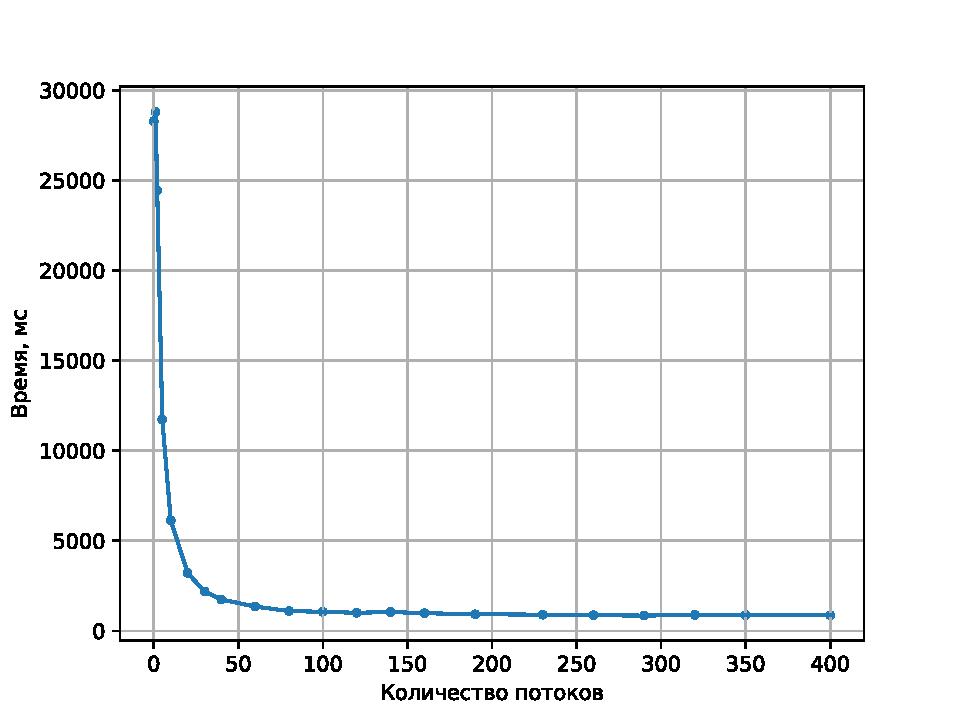
\includegraphics[scale=0.9]{../scripts/plot.pdf}
    \caption{Зависимости среднего количества запросов в секунду от количества потоков}
    \label{img:plot}
\end{figure}